%% =====================================================================
%% Overload as a Cusp Catastrophe. IEEE conference format (IEEEtran).
%% Compile: pdflatex main && bibtex main && pdflatex main && pdflatex main
%% Long-form supplement lives in ../supplement/. Full journal draft is
%% preserved as main_full_journal.tex.
%% =====================================================================
\documentclass[conference]{IEEEtran}

\usepackage{amsmath,amssymb,amsthm}
\usepackage{graphicx}
\usepackage{booktabs}
\usepackage[hidelinks]{hyperref}
\usepackage{siunitx}
% orcidlink draws the small ORCID logo next to the author name.
% Degrade gracefully if the package is not installed.
\IfFileExists{orcidlink.sty}{\usepackage{orcidlink}}%
  {\newcommand{\orcidlink}[1]{}}

\graphicspath{{./}{figures/}{../figures/}}

\newtheorem{proposition}{Proposition}
\DeclareMathOperator{\Var}{Var}
\newcommand{\dd}{\mathrm{d}}

\begin{document}

\title{Overload as a Cusp Catastrophe: Identifiability Limits and a
Ground-Truth Failure of Early-Warning Indicators in Wearable Physiology}

\author{\IEEEauthorblockN{Neil Thomas Mathew\,\orcidlink{0009-0001-8802-7376}}
\IEEEauthorblockA{Department of Computer Applications\\
CHRIST (Deemed to be University), Bengaluru, India\\
ORCID: \href{https://orcid.org/0009-0001-8802-7376}{0009-0001-8802-7376}}}

\maketitle

\begin{abstract}
Sensory and executive overload is usually modelled by labelling states and
counting transitions between them. Models of that kind fit any data and predict
nothing that could refute them. We derive overload instead from the geometry of
a cusp catastrophe. A latent load coordinate relaxes in a quartic potential
whose asymmetry follows momentary demand and whose bistability follows a slow
recovery-debt variable, so the discrete functional states become metastable
basins and the transition kernel follows from Kramers escape rates. Two
exponents are fixed in advance: hysteresis width grows as the $3/2$ power of the
splitting factor, and near the fold the variance and log-autocorrelation scale
as $\mp 1/2$ in distance to the tipping point. Conditional on the slow variable
the drift is linear in a reparameterised coefficient vector, so estimation
reduces to profiled least squares and is exact. Three results follow, and two of
them concern method rather than physiology. First, a Monte Carlo study over
$3.6\times10^{3}$ simulated series shows that at the series lengths wearable
corpora actually supply only the relaxation rate and the diffusion coefficient
are identified; the control parameters that carry the geometry are not, which
bounds what any cusp analysis of such data can claim. Second, the rolling-window
autocorrelation and variance indicators used throughout the early-warning
literature return exponents of the wrong sign on data simulated from a model
that genuinely contains a fold, so we withdraw our own early-warning test rather
than report it. Third, across 147 recordings from 40 people in three open
corpora, the one identifiable prediction is not supported above a
surrogate-calibrated null. Measured power bounds this to excluding strong and
moderate dynamics. The work is motivated by autistic adults; none are analysed
here, and a pre-registered validation is specified.
\end{abstract}

\begin{IEEEkeywords}
Critical transitions, cusp catastrophe, hysteresis, early-warning signals,
identifiability, electrodermal activity, wearable sensing, sensory overload.
\end{IEEEkeywords}

% =====================================================================
\section{Introduction}

Autistic adults describe functional breakdown under combined sensory and
cognitive demand in consistent terms: it arrives suddenly, and it clears slowly
\cite{maclennan2022}. Adult cohort studies couple sensory atypicality to
executive difficulty with large effect sizes \cite{kiep2025,demetriou2018}, so
the phenomenon is not in doubt. What is missing is a formal account of the
dynamics.

Existing models do not supply one. Computational work on autism is dominated by
Bayesian and predictive-coding framings whose empirical support a ten-year
review found mixed and methodologically inconsistent \cite{chrysaitis2023}, and
the most recent dynamical treatment of symptom trajectories is explicitly
theoretical and collects no data \cite{adamou2026}. Applied state-transition
work typically assigns states from experimental condition labels and then counts
a transition matrix, which is close to circular: the recovered matrix largely
re-describes the block structure of the protocol, and yields no prediction that
observation could contradict.

We take a different route. Rather than positing states and fitting transitions
between them, we posit a one-dimensional stochastic relaxation in a cusp
potential and let the phenomenology follow. The load coordinate $x_t$ sits in
$V(x;a,b)=\tfrac14 x^4-\tfrac12 a x^2-bx$, where the normal factor $b_t$ carries
momentary demand and the splitting factor $a_t$ carries depleted regulatory
capacity. The substantive claim is that capacity does not add to load. It
changes the geometry. Below a critical $a$ the load tracks demand and returns;
above it a second attractor appears, and with it a fold, a hysteresis loop and
critical slowing down. Sudden onset and slow recovery stop being observations to
report and become consequences to check, and because the geometry is closed-form
those consequences are numerical exponents that data can reject. This paper is
about how far that promise survives contact with real wearable data.

\noindent\textbf{Contributions.}
\begin{enumerate}
\item A cusp formulation in which the five functional states are geometric
regions rather than labels, and the $5\times5$ transition kernel is generated by
nine interpretable parameters instead of twenty counted frequencies
(Sec.~\ref{sec:model}).
\item An exact profiled-least-squares estimator, and a high-replication
identifiability study showing which parameters are recoverable at the series
lengths wearable corpora supply (Sec.~\ref{sec:ident}), which bounds every claim
such an analysis can make, including ours.
\item A ground-truth demonstration that the standard early-warning indicators
report the wrong sign on data containing a genuine fold, plus a measurement of
the eightfold size inflation of the nominal test on near-unit-root series
(Sec.~\ref{sec:results}).
\item A calibrated null on 147 recordings, with power characterised so the
result is a bound rather than an absence.
\end{enumerate}

\noindent The target population is autistic adults. No public wearable dataset
of that group exists at the temporal density this model needs
\cite{cano2024,chen2025ema}, so none are analysed here, and we say so rather
than title the work after a group it does not measure.

% =====================================================================
\section{The Cusp--Hysteretic Model}
\label{sec:model}

\begin{figure*}[t]
\centering
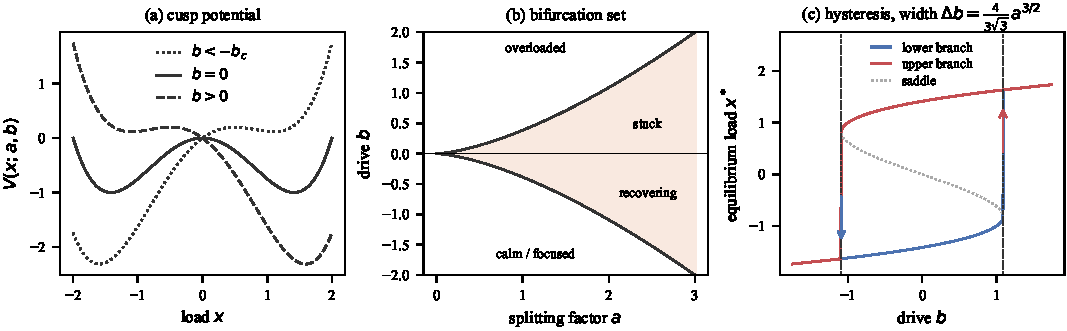
\includegraphics[width=0.94\textwidth]{fig1_geometry}
\caption{The geometry from which everything else follows. (a) The cusp potential
at three levels of drive $b$. (b) The bifurcation set in the $(a,b)$ plane, with
the five functional states appearing as regions rather than as assigned labels.
(c) The hysteresis loop, whose width is fixed by \eqref{eq:hyst} rather than
merely being positive.}
\label{fig:geometry}
\end{figure*}

\subsection{Fast dynamics and a slow debt variable}
The latent load obeys a gradient relaxation with additive noise,
\begin{equation}
\dd x_t=\lambda\!\left[-x_t^3+a_tx_t+b_t\right]\!\dd t+\sigma\,\dd W_t ,
\label{eq:sde}
\end{equation}
with control parameters linked to observed drivers and to a slow variable $A_t$
that accumulates recovery debt:
\begin{align}
b_t&=\beta_0+\beta_SS_t+\beta_TT_t+\beta_UU_t, \quad a_t=\alpha_0+\alpha_AA_t,\\
\dd A_t&=\varepsilon\!\left[\mathrm{sp}(x_t-x_{\text{ref}})-A_t\right]\!\dd t,
\qquad \varepsilon\ll1 .
\end{align}
Here $\mathrm{sp}$ is a softplus, $S_t$, $T_t$ and $U_t$ are sensory,
task-switch and uncertainty drivers, and $\lambda$ sets the timescale without
touching the geometry. Load above baseline accrues debt, debt raises $a_t$, and
a higher $a_t$ widens the hysteresis loop, so one episode makes the next easier.
That is a mechanistic reading of the refractory period qualitative accounts
describe.

\subsection{Folds and two scaling laws}
Equilibria solve $x^3-ax-b=0$. Its discriminant $4a^3-27b^2$ is positive exactly
when two stable basins coexist. Folds occur where $V''(x)=0$, that is at
$x_\pm=\pm\sqrt{a/3}$, giving critical drives $\pm b_c(a)$ with
$b_c(a)=\tfrac{2}{3\sqrt3}a^{3/2}$.

\begin{proposition}[Hysteresis width, P1]\label{prop:hyst}
For $a>0$ the system jumps to the upper branch at $b=+b_c$ and returns at
$b=-b_c$, so the loop has width
\begin{equation}
\Delta b(a)=\tfrac{4}{3\sqrt3}\,a^{3/2}.
\label{eq:hyst}
\end{equation}
\end{proposition}

Linearising \eqref{eq:sde} about a stable equilibrium gives a relaxation rate
$\lambda_{\text{rel}}=3x^{*2}-a$, which vanishes at a fold. Critical slowing
down is therefore a theorem here rather than an assumption. Writing
$\mu=b_c-b$ for the distance to the fold, the normal form gives
$\lambda_{\text{rel}}\propto\mu^{1/2}$, hence

\begin{proposition}[Early-warning exponents, P2]\label{prop:ews}
$\Var(x)\propto\mu^{-1/2}$ and $-\log\mathrm{AC1}\propto\mu^{+1/2}$.
\end{proposition}

These are point hypotheses about exponents. They differ in kind from the usual
directional claim that an indicator rises before a transition, which the
sceptical literature shows arises spuriously on almost any autocorrelated series
\cite{ditlevsen2010,boettiger2012}.

\subsection{States and transition kernel}
Crossing basin membership with the bistability condition partitions the $(a,b)$
plane into five regions (Fig.~\ref{fig:geometry}b): \emph{calm} and
\emph{focused} in the lower basin when monostable, \emph{stuck} in the lower
basin while an overloaded attractor coexists, \emph{overloaded} in the upper
basin, and \emph{recovering} in the upper basin once demand has fallen below the
level that would have put the system there. The last two are the useful ones.
Qualitative work uses both words freely, and to our knowledge neither has
previously had a precise mathematical meaning. Between-basin moves are
noise-induced escapes with Kramers rate
$r=\tfrac{1}{2\pi}\sqrt{|V''(x^*)V''(x_s)|}\exp(-2\Delta V/\sigma^2)$
\cite{kramers1940}, so the kernel is a deterministic function of
$(a_t,b_t,\sigma)$: twenty counted probabilities replaced by nine interpretable
parameters that move with demand.

% =====================================================================
\section{Materials and Methods}
\label{sec:methods}

\subsection{Corpora}
Three open corpora, each taken from its primary repository rather than a mirror,
span a gradient of experimental control: WESAD, 15 subjects in a controlled
laboratory protocol \cite{schmidt2018wesad}; Wearable Exam Stress, 10 students
across 30 examinations \cite{amin2022exam}; and Nurse Stress, 15 nurses across
roughly \SI{1250}{\hour} of hospital shifts \cite{hosseini2022nurse}. All supply
Empatica E4 electrodermal activity, blood volume pulse, skin temperature and
accelerometry. After windowing and quality screening this gives \textbf{147
recordings from 40 people}, median 194 windows each.

\subsection{Sensor assignment and a negative control}
Reading the load coordinate and its drivers from the same sensor would make the
model unfalsifiable, since shared measurement noise alone could produce apparent
coupling, so the two are assigned to disjoint sensors. The load coordinate of a
slow relaxation process must itself be slow, which is measurable rather than a
matter of preference: at a \SI{30}{\second} window tonic electrodermal activity
has lag-1 autocorrelation $0.98$, whereas a cardiac index built from heart rate
and RMSSD has $0.19$, because RMSSD over so few beats is dominated by
beat-detection error. Configuration B (tonic EDA) is therefore primary,
configuration C (skin temperature) is a robustness check, and configuration A
(the cardiac index) is retained as a \emph{negative control} in which a working
pipeline should find nothing.

\subsection{Estimation}
Taking the Euler map of \eqref{eq:sde} as the model, rather than as an
approximation to it, makes the transition density exactly Gaussian and removes
discretisation bias. Expanding the drift, the mean increment is linear in a
reparameterised coefficient vector,
\begin{equation}
\Delta x_t=\theta_1(-x_t^3)+\theta_2 x_t+\theta_3A_tx_t+\theta_4
+\theta_5S_t+\theta_6T_t+\theta_7U_t+\eta_t ,
\label{eq:linear}
\end{equation}
with $\theta_1=\lambda$, $\theta_2=\lambda\alpha_0$, $\theta_3=\lambda\alpha_A$
and $\theta_{4:7}=\lambda\beta_{0:U}$. Since $A_t$ depends only on
$\varepsilon$, the fit is ordinary least squares profiled over a single scalar:
exact, with no bounds, no starting values and no local optima. We impose
$\theta_1\ge0$, because a negative value places the system outside the model
rather than merely fitting it badly, and we retain units where that constraint
binds so that no reported proportion is conditioned on its own outcome.

\subsection{Nulls}
The nominal $t$-test on $\theta_1$ is not usable here: tonic EDA is close to a
unit-root process, and regressing on an integrated series inflates significance
in the classical way. Every test is therefore calibrated against surrogate
ensembles, both random-walk surrogates matched on length, increment variance and
marginal scale, and amplitude-adjusted Fourier surrogates (IAAFT
\cite{schreiber1996}) that preserve spectrum and marginal so only nonlinearity
can drive a rejection. Competing models (homogeneous Markov, covariate logistic,
Gaussian HMM, the nested Ornstein--Uhlenbeck case, gradient boosting) are scored
by held-out one-step predictive log-density.

% =====================================================================
\section{What This Data Can and Cannot Identify}
\label{sec:ident}

Before testing anything we asked which parameters are recoverable at the series
lengths on offer. This is not a formality. It turned out to be the result that
organises the rest of the paper.

We simulated from the model with randomised true parameters and refitted, 600
replicates at each of six lengths, then correlated true against estimated values
(Table~\ref{tab:ident}, Fig.~\ref{fig:ident}a). At $n=1000$ most parameters are
at least moderately recovered. At $n=200$, which is the median length in these
corpora, only two are: the relaxation rate $\lambda$ at $r=0.91$ and the
diffusion coefficient $\sigma$ at $r=0.95$. The splitting factor $\alpha_0$ sits
at $r=0.06$, the debt gain $\alpha_A$ at $r=-0.07$, and the slow rate
$\varepsilon$ at $r=0.07$.

\begin{figure}[t]
\centering
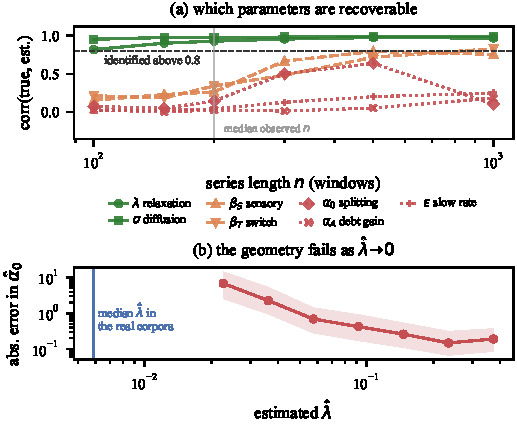
\includegraphics[width=\columnwidth]{fig9_identifiability}
\caption{(a) Recovery correlation against series length, 600 replicates per
point. Only $\lambda$ and $\sigma$ clear a useful threshold at the median
observed length. (b) The failure mechanism: absolute error in the recovered
splitting factor rises as $\hat\lambda$ falls, because $a=\theta_2/\theta_1$.
The median $\hat\lambda$ in the real corpora lies below the whole simulated
range.}
\label{fig:ident}
\end{figure}

\begin{table}[t]
\caption{Correlation between true and estimated parameters, 600 replicates per
cell. At the median observed length ($n=200$) only $\lambda$ and $\sigma$ are
identified. The control parameters carrying the geometry require $n\gtrsim500$.}
\label{tab:ident}
\centering
\begin{tabular}{@{}lrrrr@{}}
\toprule
Parameter & $n=100$ & $n=200$ & $n=500$ & $n=1000$ \\
\midrule
$\lambda$ (relaxation rate) & $0.82$ & $\mathbf{0.91}$ & $\mathbf{0.98}$ & $\mathbf{0.97}$ \\
$\sigma$ (diffusion)        & $0.96$ & $\mathbf{0.95}$ & $\mathbf{0.99}$ & $\mathbf{0.99}$ \\
$\beta_S$ (sensory drive)   & $0.33$ & $0.22$ & $0.80$ & $0.65$ \\
$\beta_T$ (task switch)     & $0.21$ & $0.26$ & $0.74$ & $0.82$ \\
$\alpha_0$ (splitting)      & $0.02$ & $0.06$ & $0.66$ & $0.59$ \\
$\alpha_A$ (debt gain)      & $0.05$ & $-0.07$ & $0.07$ & $0.16$ \\
$\varepsilon$ (slow rate)   & $0.01$ & $0.07$ & $0.21$ & $0.27$ \\
\bottomrule
\end{tabular}
\end{table}

The consequence is sharp, and it applies to any study of this kind rather than
only to ours. The recovered geometry is built from the ratios
$a=\theta_2/\theta_1$ and $b=\theta_4/\theta_1$, so when $\hat\lambda$ is small
both inflate without bound (Fig.~\ref{fig:ident}b). That is exactly what the
real fits show: among units where the constraint does not bind, the median
$\hat\lambda$ is $0.0059$ and the median recovered $\hat\alpha_0$ is $12$, which
would place the attractors near $\pm2$ on a coordinate standardised to unit
variance. Those are not weakly bistable systems. They are systems with no
restoring cubic term, whose apparent geometry comes from dividing by a number
close to zero. Note that this median $\hat\lambda$ falls below the entire range
our simulation covers, so the real recordings sit further into the
non-identified regime than any of the $3.6\times10^{3}$ synthetic series we used
to characterise it.

So exactly one of the five pre-stated predictions is evaluable here: the
existence of the restoring cubic term, governed by the one well-identified
parameter. P1 needs the ratio of two poorly identified quantities, P2 the fold
distance, and P3 to P5 depend on $\varepsilon$ and $\alpha_A$. We report that
structure rather than four numbers that would look like tests.

% =====================================================================
\section{Results}
\label{sec:results}

\begin{figure}[t]
\centering
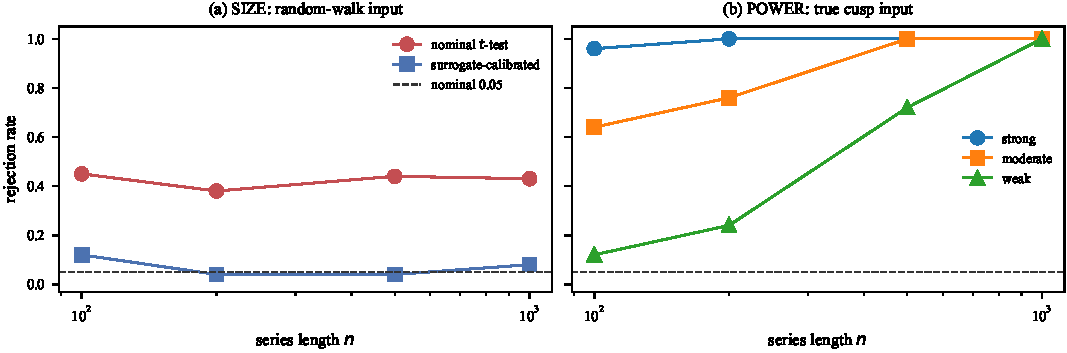
\includegraphics[width=\columnwidth]{fig7_power_size}
\caption{(a) Size on random-walk input. The nominal test rejects at roughly
$0.42$ irrespective of series length, while surrogate calibration restores
approximately nominal size. (b) Power of the calibrated test on input that
genuinely contains a cusp. At the median observed length, strong and moderate
dynamics are detected and weak dynamics largely are not.}
\label{fig:powersize}
\end{figure}

\subsection{The nominal test is invalid; the calibrated one is adequately powered}
Over $12{,}000$ random-walk replicates spanning six lengths, the nominal
one-sided $t$-test on $\theta_1$ rejects $42.0\%$ of the time rather than $5\%$.
The inflation does not shrink with sample size. It grows, from $36.8\%$
($95\%$ CI $[34.7,38.9]$) at $n=100$ to $44.4\%$ $([42.2,46.5])$ at $n=1000$,
which is the signature of spurious regression on an integrated series rather
than a small-sample artefact. Surrogate calibration restores nominal size across
the same grid: $5.7\%$ pooled over $3{,}000$ calibrated replicates, with every
per-length interval covering $0.05$. Calibration costs power, so we quote power
for the test actually used. At $n=200$ it is $1.00$ for strong cusp dynamics,
$0.76$ for moderate and $0.24$ for weak, reaching $1.00$ in every regime by
$n=1000$ (Fig.~\ref{fig:powersize}). The null below therefore excludes strong
and moderate dynamics. It does not exclude a faint fold.

\subsection{The standard early-warning estimator fails on ground truth}
Proposition~\ref{prop:ews} is a statement about the system. Testing it requires
an estimator, and we checked ours before trusting it. Simulating from a model
that genuinely contains a fold, the exponent computed from the true equilibrium
curvature is $+0.565$ against a predicted $+0.5$, so theory and implementation
agree. The rolling-window indicators that the early-warning literature relies on
\cite{scheffer2009,dakos2012} do not. Across a grid of window lengths,
detrending choices and series lengths up to $n=20{,}000$, rolling
$-\log\mathrm{AC1}$ returns negative slopes where $+0.5$ is predicted and
rolling variance returns positive slopes where $-0.5$ is predicted
(Table~\ref{tab:ewsval}).

The mechanism is structural, not statistical. Critical slowing down means the
relaxation time diverges at the fold, so a fixed-width window saturates
precisely where the effect is strongest, and detrending removes the
low-frequency power carrying what remains. Raising $n$ by an order of magnitude
does not recover the sign. We therefore withdraw our own P2 test as
uninterpretable, and the caution generalises: a directional early-warning result
obtained this way is weak evidence either way.

\begin{table}[t]
\caption{Can the standard early-warning estimator recover the exponent on
ground-truth cusp data? The closed-form theory does. The rolling-window
estimators return the wrong sign.}
\label{tab:ewsval}
\centering
\begin{tabular}{@{}lcccr@{}}
\toprule
Estimator & Predicted & Detrend & Window & Median \\
\midrule
theory $\lambda_{\text{rel}}(\mu)$ & $+0.5$ & --- & --- & $\mathbf{+0.565}$ \\
\midrule
$-\log$AC1 & $+0.5$ & no  & 30  & $-0.262$ \\
$-\log$AC1 & $+0.5$ & no  & 120 & $-0.035$ \\
variance   & $-0.5$ & no  & 30  & $+0.311$ \\
variance   & $-0.5$ & yes & 120 & $+0.036$ \\
\bottomrule
\end{tabular}
\end{table}

\subsection{The identifiable prediction is not supported}
Under the calibrated test, the restoring cubic term is significant in $2.7\%$ of
the 147 units, against a nominal $5\%$. By corpus the figures are $0.0\%$ for
WESAD ($n=15$), $0.0\%$ for the examination sessions ($n=30$) and $3.9\%$ for
the nurse sessions ($n=102$). Because 102 units come from 15 nurses, we also
weight one vote per person, which gives $1.5\%$ (Wilson interval $[0.0,3.1]\%$),
with $10\%$ of people showing at least one significant session. That last figure
is the most generous reading available and is still what chance produces across
several sessions each.

Held-out prediction agrees from a different direction. The full model does not
beat its own nested monostable special case: it wins on $33.8\%$ of units, with
a median difference of $-0.25$ nats per step and a Wilcoxon $p=8\times10^{-5}$
in the simpler model's favour. Since the monostable model is this model with the
cubic term switched off, that is the cleanest available statement that the cubic
term is doing no work. Prospective onset prediction gives AUC between $0.50$ and
$0.46$ at lead times of 3 to 12 windows, which is chance.

\subsection{Structure without fold structure}
The null is specific, and it would be wrong to summarise it as noise. Two of the
three statistics we calibrate do exceed their surrogate nulls: the likelihood
ratio against the monostable restriction at $40.8\%$ of units, and the
bimodality of the marginal distribution at $49.7\%$. Only the statistic that
isolates the cubic term sits at chance. A bimodal marginal accompanied by no
cubic drift is exactly the configuration in which a study reporting
distributional evidence alone would conclude the opposite of the correct answer.

Robustness is mixed, and we report it that way. Configuration B sits at nominal
under both the random-walk ($0.046$) and the harder IAAFT ($0.069$) ensembles,
and holds across \SIrange{30}{120}{\second} windows. Configurations A and C are
elevated, at $0.11$ to $0.16$. Three explanations were tested and all failed:
IAAFT did not bring C down, clipping rates run opposite to the effect, and a
size study on AR(1) series ($\phi$ from $0$ to $1$) found no persistence at
which the calibrated test over-rejects. What remains is nonlinear structure the
surrogates do not reproduce. Since A is the negative control, built on a
coordinate already shown to be noise-dominated, the parsimonious reading is
artefact from motion and peak-detection failure rather than a fold. A test that
fires on the negative control shows that significance does not mean cusp there,
which is why the conclusion rests on B.

% =====================================================================
\section{Discussion and Conclusion}

Modelling overload as motion in a cusp potential replaces a descriptive account
with a generative one whose consequences are computable in advance. States
become basins, the kernel becomes a function of nine parameters, and sudden
onset, delayed recovery and two exponents become point hypotheses. The cost of
that precision is that the model can lose, and here it did.

The identifiability result is the more durable contribution. Any attempt to fit
cusp geometry to wearable physiology inherits the same ratio structure, so such
a study needs either much longer records, on the order of $n\gtrsim500$ windows,
or a reparameterisation that estimates $a$ and $b$ directly. Reporting a
splitting factor of 12 from a 200-window recording is not a finding, and the
arithmetic that produces it is not specific to our implementation.

\emph{Limitations.} No autistic participants are analysed, so the motivating
claim is untested rather than refuted. Tonic electrodermal activity is a
peripheral, artefact-prone proxy for a latent construct. Weak cusp dynamics
remain compatible with our data. The estimator critique covers fixed-width
rolling indicators with and without Gaussian detrending, which is what the
applied literature mostly uses, and does not extend to adaptive-bandwidth or
spectral estimators, which we did not test.

\emph{Toward validation.} We pre-specify the study that would test the mechanism
in its intended population: 28 days of ecological momentary assessment with
continuous wrist physiology in autistic adults and a matched comparison group,
using the same estimator, nulls and falsification criteria as here. The primary
hypothesis is a between-group difference in $\alpha_0$, better powered than the
within-group detection attempted here, and the design targets $n\gtrsim500$
windows per participant so the control parameters sit inside the identifiable
regime. A second well-powered null under those conditions would be evidence that
overload is not a cusp catastrophe at physiological timescales.

\section*{Acknowledgment}
This work uses the WESAD, Wearable Exam Stress and Nurse Stress datasets, and I
thank their authors for releasing them openly. In accordance with IEEE policy on
generative AI, the author discloses that an AI assistant was used for code
implementation, literature organisation and manuscript drafting. The author
verified all analyses, results and claims, and is solely responsible for the
content.

\bibliographystyle{IEEEtran}
\bibliography{refs}

\end{document}
